\chapter{Quantum Channel Model for SPADE}
\label{ch:exoplanet_experiment}

Chapter~\ref{ch:astrophysical_theory} introduced SPADE.  This project first asked if experimental data provided by \textbf{ASI Matera} could support the truncated-QFI methods of Chapter~\ref{ch:methods}~\cite{Santamaria2024single}.  Access to low-order Hermite--Gauss modes suggested a possible link to the dominant spectral information required by TQFI.  Section~\ref{sec:spade_question_record} develops this link as the proposed VQ-SPADE scheme.

The experiment had already ended when the data became available.  Its aggregate first-order counts could not support the required variational protocol or an experimental TQFI calculation.  This limitation led to a change in perspective.  A classical model was first fitted to the observed counts, after which the full experiment was organized as a sequential quantum-to-classical channel model.  The data constrain its population-level projection (the diagonal elements), while the assumed quantum model provides checkpoints for conditional QFI and CFI calculations.

This channel sequence is the main outcome of the experimental study.  It lays the foundation for future SPADE experiments.  A new collaboration with ASI Matera could collect the measurements needed to calibrate the channel and then test VQ-SPADE with a programmable mode transformation.

\begin{remark}[Chapter Summary]
    The quantum-channel framework provides a physically complete and modular description of the experiment and enables conditional QFI calculations.  The current aggregate-count data constrain only its population-level classical projection.  They do not reconstruct the complete quantum channel or its coherence dynamics.
\end{remark}



\begin{infobox}[sec:spade_question_record]{The proposed VQ-SPADE as an optical VQSE}

    The initial intuition was that low-order SPADE outcomes might provide the dominant spectral information needed by TQFI.

    \faLightbulb \hspace{5pt} Fixed HG outcome probabilities do not generally equal the eigenvalues of the optical state because the state need not be diagonal in the HG basis.\footnote{More precisely, the eigenvalue vector of the state majorizes the vector of HG-basis probabilities.} A trainable unitary can rotate the state's eigenbasis onto the fixed HG measurement basis, so the output probabilities equal the eigenvalues at the ideal optimum.

    We call this proposed variational extension VQ-SPADE.  It was not part of the completed experiment.  VQ-SPADE would use SPADE as the measurement stage of an optical VQSE.  A programmable coherent mode transformation $V(\boldsymbol\beta)$ would play the role of the trainable unitary in Section~\ref{sec:vqse_deep_dive}.  Resolved SPADE ports would replace the computational-basis measurement.  For an optical state $\rho(d_a)$, the measured probabilities would be
    \begin{equation}
        p_k(\boldsymbol\beta;d_a)
        =\langle HG_k|V(\boldsymbol\beta)\rho(d_a)
        V^\dagger(\boldsymbol\beta)|HG_k\rangle
        \label{eq:spade_optical_vqse_probabilities}
    \end{equation}
    A classical optimizer would minimize a weighted VQSE cost built from these probabilities.  The majorization relation in Eq.~\eqref{eq:vqse_majorization} connects this cost to the dominant eigenvalues.  At an ideal optimum, the transformation would satisfy
    \begin{equation}
        V(\boldsymbol\beta_{\mathrm{opt}})|\lambda_k(d_a)\rangle
        =e^{i\phi_k}|HG_k\rangle
        \qquad
        p_k(\boldsymbol\beta_{\mathrm{opt}};d_a)=\lambda_k(d_a)
        \label{eq:spade_optical_vqse_mapping}
    \end{equation}
    The resolved output frequencies would then estimate the dominant eigenvalues.  The inverse transformation $V^\dagger(\boldsymbol\beta_{\mathrm{opt}})$ would map the HG mode states back to the corresponding eigenvectors.  The HG modes are therefore output labels, not assumed eigenvectors of the incoming state.  This result requires a mode transformation flexible enough to reach the eigenbasis and a complete measurement of the finite set of modes used in the model.  Probability outside that set must remain as a complement outcome.

    This diagonalization would give the dominant eigenvalues and eigenvectors of $\rho(d_a)$.  TQFI also depends on the nearby state $\rho(d_a+\Delta)$.  In the notation of the VQFIE procedure in Algorithm~\ref{alg:vqfie}, the required quantities include
    \begin{equation}
        M_{ij}
        =\langle\lambda_i(d_a)|\rho(d_a+\Delta)|\lambda_j(d_a)\rangle
        \label{eq:spade_tqfi_required_overlaps}
    \end{equation}
    An optical implementation would therefore require fresh copies of both states, a controllable modal transformation, resolved and normalized SPADE outcomes, and extra overlap or interferometric measurements.  The eigenbasis can depend on the source parameters.  The transformation could therefore be fixed near a calibrated operating point or updated adaptively.

    The experiment did not scan programmable transformations.  The stored aggregate $HG_{01}+HG_{10}$ counts also lack the resolved probabilities and matrix elements required by this protocol.  VQ-SPADE is therefore a proposal for a future experiment, not a result extracted from the present data.
\end{infobox}

\subsection{The low-mode link and three distinct reductions}

The motivation for this proposal comes from the low-order SPADE receiver in Chapter~\ref{ch:astrophysical_theory} and the rank-truncation methods in Chapter~\ref{ch:methods}.  A displaced point-spread function has support in an infinite-dimensional HG space, but its lowest orders carry most of the displacement response near alignment.  This makes a low-mode implementation possible, but it does not make an HG cutoff equal to a rank truncation.  Three different reductions must be kept separate.

\paragraph{Numerical HG cutoff.}
A numerical cutoff approximates the infinite-dimensional source model by keeping HG modes up to a chosen order.  Its accuracy is checked by increasing the cutoff until the calculated quantities converge.  It is a computational approximation, not a restriction imposed by SPADE.

\paragraph{Accessible-mode channel.}
SPADE gives access to a fixed set of modes.  A model of this restriction must keep the probability outside that set as a complement or failure outcome.  For a selected subspace with projector $P_M$, we use the following flagged channel.
\begin{equation}
    \mathcal{E}_M(\rho)
    =P_M\rho P_M
    +\operatorname{Tr}\!\left[(\mathbb{I}-P_M)\rho\right]
    |\mathrm{fail}\rangle\langle\mathrm{fail}|
    \label{eq:spade_accessible_projection}
\end{equation}
The failure flag keeps the probability in unobserved modes.  Discarding this probability and renormalizing $P_M\rho P_M$ would introduce postselection and could overstate the available information.

\paragraph{Rank-$m$ TQFI.}
Rank-$m$ TQFI instead keeps the $m$ dominant eigenvectors of the parameterized density operator.  These state-dependent eigenvectors do not have to match the HG modes selected by the apparatus.  This reduction therefore requires access to the dominant eigenspace rather than only a chosen set of detector ports.

\subsection{Dataset description: the count \enquote{cube}}

The recorded observable is
\begin{equation}
    n_1=n_{HG_{01}}+n_{HG_{10}}
    \qquad
    \texttt{data}[d_a,\epsilon,r]=n_{1,r}
    \label{eq:spade_recorded_count}
\end{equation}
Here $d_a=d/w_0$ is the signed nominal displacement, $\epsilon$ is the faint-source intensity over the bright source defined in Eq.~\eqref{eq:intensity_ratio_epsilon}, and $r$ indexes repetitions.  The cube contains $21\times25\times100=52{,}500$ integer counts.  It covers $d_a\in[-0.66667,0.66667]$ and $\epsilon\in[0.00427,0.09593]$, with $100$ independent $10\,\mathrm{ms}$ repetitions at every setting.  Figure~\ref{fig:spade_count_data} shows one repetition and the mean over all repetitions.

\begin{figure}[htbp]
    \centering
    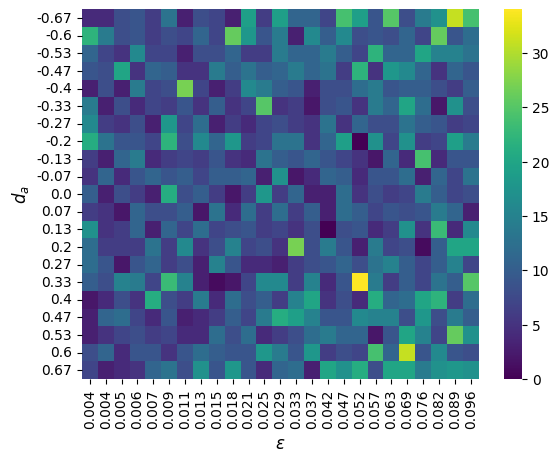
\includegraphics[width=0.43\textwidth]{figures/asi_report/sample_1_exoplanet_2026.png}
    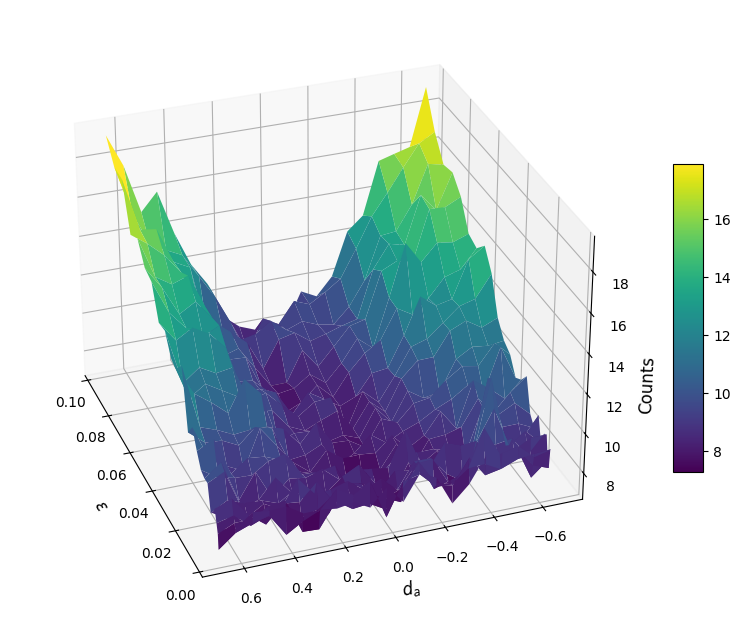
\includegraphics[width=0.52\textwidth]{figures/asi_report/average_sample_exoplanet_2026.png}
    \caption{Sample and average SPADE count data for the exoplanet experiment.  The left panel shows a single repetition, while the right panel shows the average over all repetitions.}
    \label{fig:spade_count_data}
\end{figure}

The count cube provides the aggregate $n_1$ at every nominal $(d_a,\epsilon)$ setting, together with the signed scan spatial coordinates and source fractions.  The repetitions support estimates of setting means, variances, and empirical uncertainties.  The record does not include simultaneous $HG_{00}$ counts, separate $HG_{01}$ and $HG_{10}$ streams, higher-order modes, the complement, or no-click events.  It also lacks incident-flux monitoring, source-blocked background, timestamps, detector diagnostics, and a complete mode-injection transfer matrix.  Appendix~\ref{app:spade_diagnostics} gives the detailed raw-count diagnostics and exposure checks.

The missing outcomes limit the analysis.  Separate $HG_{01}$ and $HG_{10}$ counts would resolve two orthogonal first-order directions.  Recording $HG_{00}$ together with aggregate $HG_1$ would provide a reference and a separation-sensitive outcome.  A nonzero $n_1$ at $d_a=0$ can combine background, bright-mode leakage, coupling variation, alignment error, and higher-order leakage.  Dividing $n_1$ by an assumed photon number and setting $p_0=1-p_1$ would hide these contributions in the remainder.  The data also contain no phase-sensitive observable and therefore cannot determine off-diagonal HG coherences.  The record supports the usual statistical forward count models, not optical-state reconstruction or quantum process tomography.

% ==============================================================================
\section{The Sequential Quantum-to-Classical Model}
\label{sec:spade_sequential_channels}
% ==============================================================================

We use the density-operator, quantum-channel, and POVM conventions introduced in Chapter~\ref{ch:MathBackground}.  Appendix~\ref{app:mathematical_background} gives further details on generalized measurements.  Here we specify only the physical action and experiment-specific parameters of each channel.

Figure~\ref{fig:channel_stages} shows the full ordering of the model.

\begin{figure}[H]
    \centering
    {
        \tikzset{
            spade preparation/.style={draw, thick, rounded corners},
            spade quantum/.style={draw, thick, fill=gray!12},
            spade measurement/.style={draw, very thick, rounded corners, fill=gray!28},
            spade classical/.style={draw, densely dashed}
        }
        \begin{tikzcd}[
                row sep=0.32cm,
                cells={nodes={rectangle, inner xsep=8pt, inner ysep=4pt, font=\small}}
            ]
            |[spade preparation]| \text{Source preparation} \arrow[d] \\
            |[spade quantum]| \text{Survival or erasure} \arrow[d] \\
            |[spade quantum]| \text{Displacement, alignment errors} \arrow[d] \\
            |[spade quantum]| \text{HG-basis dephasing} \arrow[d] \\
            |[spade quantum]| \text{Coherent HG-mode mixing} \arrow[d] \\
            |[spade quantum]| \text{Mode-dependent loss into a failure sector} \arrow[d] \\
            |[spade quantum]| \text{Flagged accessible-mode reduction} \arrow[d] \\
            |[spade measurement]| \text{Limited-outcome SPADE measurement} \arrow[d] \\
            |[spade classical]| \text{Classical readout, cross-talk} \arrow[d] \\
            |[spade classical]| \text{Background and calibration variation} \arrow[d] \\
            |[spade classical]| \text{Repeated-count model}
        \end{tikzcd}
    }
    \caption{The quantum-to-classical sequence used to model the SPADE experiment. The rounded unshaded box marks state preparation. Light gray boxes mark pre-measurement quantum channels. The darker box marks the SPADE measurement. Dashed boxes mark classical post-measurement stages.}
    \label{fig:channel_stages}
\end{figure}

The SPADE measurement is the boundary between the quantum and classical parts of the model.  The preceding channels act on the optical state.  SPADE converts that state into outcome probabilities.  Readout and calibration then act on those probabilities, and the final layer describes the repeated counts.  Appendix~\ref{app:spade_diagnostics} lists the parameter source and information role of every stage.

The way we described the source raises a question about coherence.  Section~\ref{sec:weak_light_as_quantum_state} describes the star and planet as an incoherent mixture, but the displaced one-photon wavefunction can still contain coherence between HG modes.  Appendix~\ref{sec:spade_hg_coherence} explains this basis-dependent distinction.  This is why the provisional workbench includes dephasing and coherent mixing.  Their parameters are not fitted from the aggregate counts.

\subsection{Classical and quantum objects in the model}

A classical state is a probability vector $\boldsymbol p$.  To introduce a quantum channel let us choose a basis, the same probabilities can be written as a diagonal density matrix.
\begin{equation}
    \rho_{\mathrm{diag}}=\operatorname{diag}(\boldsymbol p)
    \label{eq:spade_classical_embedding}
\end{equation}
That is how a general quantum state can also contain off-diagonal coherences.\footnote{That is also why we say that a quantum state is subject to decoherence, the off-diagonal elements vanish, and it can be represented as a classical probability vector.}
A classical stochastic channel maps probability vectors to probability vectors.  A quantum channel acts on the complete density operator and can describe and change both populations and coherences.  Measurement produces a classical vector $p_y=\operatorname{Tr}(\rho M_y)$.  Detector reporting and repeated-count statistics then act on that vector.  A probability vector is not a quantum channel or a substitute for the pre-measurement state.

\faLightbulb \hspace{5pt} The main advantage of the quantum channel description is not the number of adjustable parameters, as we can think at a first glance.  It can represent coherence, interference, loss, mode mixing, and open-system dynamics while preserving positivity and normalization.  The classical layers describe what happens after measurement without treating detector effects as changes to the pre-measurement quantum state.


\subsection{Source preparation and the HG convention}

The spatial one-photon sector is not limited to two dimensions.
\begin{equation}
    \mathcal{H}_{\mathrm{spatial}}
    =\operatorname{span}\{|HG_{00}\rangle,|HG_{01}\rangle,|HG_{10}\rangle,|HG_{02}\rangle,\ldots\}
    \label{eq:spade_infinite_hg_space}
\end{equation}
For a one-photon event before apparatus loss, we use the following mutually incoherent bright/faint source state.
\begin{equation}
    \rho_S(d_a,\epsilon)
    =(1-\epsilon)|HG_{00}\rangle\langle HG_{00}|
    +\epsilon|\psi_{d_a}\rangle\langle\psi_{d_a}|
    \label{eq:spade_source_state}
\end{equation}
The sorter origin is aligned to the bright source, as in the experiment~\cite{Santamaria2024single}.  For the scan direction, the displaced state has the following expansion.
\begin{equation}
    |\psi_{d_a}\rangle
    =\sum_{n=0}^{\infty}e^{-q/2}\frac{\alpha^n}{\sqrt{n!}}|HG_n\rangle
    \qquad
    \alpha=\frac{d_a}{2}
    \qquad
    q=|\alpha|^2=\frac{d_a^2}{4}
    \label{eq:spade_effective_coordinates}
\end{equation}
The modal probabilities follow from this expansion.
\begin{equation}
    P(HG_n|\psi_{d_a})=e^{-q}\frac{q^n}{n!}
    \qquad
    p_1(d_a,\epsilon)=\epsilon q e^{-q}
    \label{eq:spade_sector_probabilities}
\end{equation}
Here $p_1$ is the ideal aggregate first-order probability for the one-axis displacement model used by the count analysis.

Even if $|\psi_{d_a}\rangle$ has nonzero amplitudes in infinitely many HG modes, the one-photon state in Eq.~\eqref{eq:spade_source_state} is a mixture of at most two pure states.  Its rank is therefore at most two.  Infinite basis support and density-matrix rank are different concepts.  The numerical cutoff check is reported in Appendix~\ref{app:spade_diagnostics}.

\subsection{Pre-measurement quantum channels}

The channels in this subsection act on the optical state before SPADE produces a classical outcome.  They describe different physical effects.  The survival channel describes loss common to all modes.  Alignment changes the position of the image relative to the sorter.  Dephasing changes HG coherences, while coherent mixing transfers amplitude between HG modes.  Mode-dependent loss then gives different transmissions to different modes.  Finally, the accessible-mode channel keeps track of light outside the measured subspace.

\paragraph{Survival or erasure.}
A photon can be lost during propagation, collection, or detection before it gives a usable SPADE outcome.  We group these common losses into a survival probability $\eta$. Here, $\eta$ is conditional on the incident-photon normalization $N_{\mathrm{in}}$. It must not be identified directly with the temporal-mode detection probability in Eq.~\eqref{eq:optical_density_matrix_chap}, which uses a different photon-number convention. If the photon survives, its one-photon state remains $\rho_S$.  If it is lost, the output is the vacuum state $|\mathrm{vac}\rangle$.  The two possibilities are represented by
\begin{equation}
    \rho_{\mathrm{surv}}
    =\mathcal{S}_{\eta}(\rho_S)
    =\eta\rho_S+(1-\eta)|\mathrm{vac}\rangle\langle\mathrm{vac}|
    \label{eq:spade_loss_channel}
\end{equation}
The first term has total probability $\eta$, while the vacuum term has probability $1-\eta$.  Their sum therefore keeps the total probability equal to one.  We assume that $\eta$ does not depend on the separation $d_a$.  Under this assumption, lost photons carry no information about $d_a$, so this channel reduces the information per launched photon.  It does not alter the state of the photons that survive.

The optical response used by the count model and the information-retention ratios is written per surviving photon. Let $\Pi_1$ project onto the one-photon sector. The normalized state conditional on common survival is
\begin{equation}
    \widetilde{\rho}_{\mathrm{surv}}
    =
    \frac{\Pi_1\rho_{\mathrm{surv}}\Pi_1}
    {\operatorname{Tr}(\Pi_1\rho_{\mathrm{surv}})}
    =\rho_S
    \qquad
    \operatorname{Tr}(\Pi_1\rho_{\mathrm{surv}})=\eta
    \label{eq:spade_conditional_survival_state}
\end{equation}
This conditioning does not discard the survival probability. The factor $\eta$ is carried into the count scale $T=N_{\mathrm{in}}\eta$. Mode-dependent loss and inaccessible modes are still kept as explicit failure outcomes later in the sequence.

The count data do not determine $\eta$ on its own because the incident photon number $N_{\mathrm{in}}$ was not recorded for each acquisition.  The data mainly constrain the product $T=N_{\mathrm{in}}\eta$.  The parameter $\eta$ is therefore not reported as a measured efficiency.

\paragraph{Alignment and displacement.}
The SPADE sorter defines the origin of the HG basis.  A fixed offset $\delta_{\mathrm{sorter}}$ means that this origin does not exactly match the origin used for the source.  The corresponding displacement is reversible and is described by a unitary transformation
\begin{equation}
    \widetilde{\rho}_{\mathrm{align}}
    =U_{\mathrm{align}}(\delta_{\mathrm{sorter}})
    \widetilde{\rho}_{\mathrm{surv}}
    U_{\mathrm{align}}^{\dagger}(\delta_{\mathrm{sorter}})
    \label{eq:spade_alignment_channel}
\end{equation}
The tilde marks a state conditional on common photon survival. The operators on the two sides of $\widetilde{\rho}_{\mathrm{surv}}$ shift both the ket and bra parts of the density operator.  Because the offset is fixed and does not depend on $d_a$, this transformation preserves state QFI.  It can still lower the CFI of a fixed SPADE receiver because the receiver is now measured in a misaligned basis.

The fitted offset $\delta$ in the empirical mean model also absorbs calibration shifts.  It is therefore not a separate measurement of $\delta_{\mathrm{sorter}}$.  Random displacement has a different meaning.  It averages over several offsets, as would happen under position jitter, and can reduce coherence.

\paragraph{HG-basis dephasing.}
The displaced optical field can be coherent across several HG modes.  Phase fluctuations may weaken the off-diagonal elements that describe this coherence without changing the probability in each mode.  We represent this effect by
\begin{equation}
    \widetilde{\rho}_{\mathrm{deph}}
    =\mathcal{D}_{v}(\widetilde{\rho}_{\mathrm{align}})
    =v\widetilde{\rho}_{\mathrm{align}}+(1-v)\operatorname{diag}_{HG}(\widetilde{\rho}_{\mathrm{align}})
    \qquad 0\leq v\leq1
    \label{eq:spade_quantum_sequence}
\end{equation}
Here $\operatorname{diag}_{HG}(\rho)$ means that the diagonal HG populations are kept and all off-diagonal HG elements are set to zero.  The value $v=1$ leaves the state unchanged.  The value $v=0$ removes all HG coherence.  Intermediate values multiply the off-diagonal elements by $v$ while leaving the modal populations unchanged.

Dephasing can reduce state QFI.  A direct measurement of HG populations cannot detect $v$ unless a later coherent operation converts coherence into a population change.  If coherent mixing follows dephasing, the final populations can depend on both processes, but the present aggregate counts cannot separate their effects.  The value of $v$ is therefore assumed only for sensitivity analysis.
Since we said that the system is modeled as an incoherent mixture, Appendix~\ref{sec:spade_hg_coherence} explains why mutually incoherent sources can still have coherence in the HG basis.

\paragraph{Coherent mode mixing.}
Optical imperfections can transfer field amplitude coherently between $HG_0$ and $HG_1$.  A unitary rotation with a mixing angle and phase describes this coupling.  The angle sets how much amplitude is exchanged, while the phase controls how the two amplitudes interfere.  A delicate distintion has to be made, since this is different from electronic cross-talk.  Coherent mixing acts on the optical amplitudes before measurement, whereas electronic cross-talk acts on the classical port labels after measurement.

If the mixing angle and phase do not depend on $d_a$, the rotation preserves state QFI.  It can still change the CFI of SPADE because it changes which populations reach the fixed measurement ports.

\paragraph{Mode-dependent loss.}
Different HG modes may pass through the apparatus with different efficiencies.  Let $\tau_j$ be the conditional transmission probability of mode $j$ after the common survival stage.  The operator
\begin{equation}
    L=\sum_j\sqrt{\tau_j}|HG_j\rangle\langle HG_j|
\end{equation}
multiplies the amplitude of mode $j$ by $\sqrt{\tau_j}$, which multiplies its probability by $\tau_j$.  The transmitted state alone has trace smaller than one.  We therefore send the missing probability to an orthogonal failure state

\begin{equation}
    \mathcal{L}_{\boldsymbol\tau}(\rho)
    =L\rho L^{\dagger}
    +\operatorname{Tr}\!\left[(\mathbb{I}-L^{\dagger}L)\rho\right]
    |\mathrm{fail}\rangle\langle\mathrm{fail}|
    \label{eq:spade_modal_loss}
\end{equation}
Here $\rho$ denotes the one-photon block conditional on common survival. In the complete unconditional description, the vacuum branch produced by Eq.~\eqref{eq:spade_loss_channel} remains vacuum. The first term is the part that passes through the apparatus.  The trace in the second term is the total probability lost from all modes.  Adding the failure state keeps the conditional output normalized.  A value $\tau_j=1$ means full transmission of mode $j$, while $\tau_j=0$ means complete loss of that mode.

Mode-dependent loss can change both accessible-state QFI and SPADE CFI.  The experiment did not provide an absolute transmission calibration for each mode.

\paragraph{Accessible-mode reduction.}
After these optical channels, the receiver accesses only a selected set of HG modes.  Equation~\eqref{eq:spade_accessible_projection} projects the optical state onto that set and places all probability outside it in the state $|\mathrm{fail}\rangle$.  This step describes a physical limit of the receiver.  It is not the numerical HG cutoff used to approximate an infinite matrix.  Keeping the failure outcome preserves normalization and avoids treating discarded photons as if they had been successfully detected.

\subsection{Measurement and post-measurement classical layers}

\paragraph{SPADE measurement.}
Using the POVM convention of Chapter~\ref{ch:MathBackground}, we specify the ideal low-order outcomes below.
\begin{align}
    M_0               & =|HG_{00}\rangle\langle HG_{00}|\nonumber \\
    M_1               & =|HG_{01}\rangle\langle HG_{01}|
    +|HG_{10}\rangle\langle HG_{10}|\nonumber                     \\
    M_{\mathrm{fail}} & =\mathbb{I}-M_0-M_1
    \label{eq:spade_imperfect_povm}
\end{align}
Let $\widetilde{\rho}_M$ denote the accessible state conditional on common survival. It includes the explicit failure outcome from mode-dependent loss and inaccessible modes. The corresponding probabilities are $\widetilde{p}_y=\operatorname{Tr}(M_y\widetilde{\rho}_M)$. A complete low-order experiment would record all three outcomes. The available record instead stores only repeated counts assigned to the coarse-grained $M_1$ result.

\paragraph{Classical readout and cross-talk.}
The POVM produces the conditional probability vector $\widetilde{\boldsymbol p}$ with components $\widetilde{p}_0$, $\widetilde{p}_1$, and $\widetilde{p}_{\mathrm{fail}}$.  Confusion between reported ports is then described by the classical stochastic channel $\widetilde{\boldsymbol p}_{\mathrm{rep}}=R\widetilde{\boldsymbol p}$.  The sequential fit uses the readout matrix below.
\begin{equation}
    R_{\chi}=
    \begin{pmatrix}
        1-\chi & \chi   & 0 \\
        \chi   & 1-\chi & 0 \\
        0      & 0      & 1
    \end{pmatrix}
    \qquad \chi=0.0035
    \label{eq:spade_readout_matrix}
\end{equation}
The value $\chi=0.0035$ is fixed externally from the paper's reported cross-talk calibration~\cite{Santamaria2024single}.  The paper does not give a complete measured transfer matrix.  The symmetric matrix and the isolation of the failure outcome are therefore assumptions.  This classical map can reduce measurement CFI, but it does not change pre-measurement QFI.

\paragraph{Calibration, background, and counts.}
In the final stages, an additive background $B$, a multiplicative coupling field $g(d_a,\epsilon)$, and a discrete repeated-count law act on the reported probability.  We use the following sequential mean.
\begin{equation}
    \mu(d_a,\epsilon)
    =B+T\,g(d_a,\epsilon)\,\widetilde{p}_{\mathrm{rep},1}(d_a,\epsilon)
    \qquad
    T=N_{\mathrm{in}}\eta
    \label{eq:spade_count_channel}
\end{equation}
Here $N_{\mathrm{in}}$ is the number of incident photons in one $10\,\mathrm{ms}$ acquisition, and $\eta$ is their common survival probability. Their product $T$ is the identifiable conditional throughput scale. The probability $\widetilde{p}_{\mathrm{rep},1}$ is conditional on survival and therefore does not contain another factor of $\eta$. Equivalently, the unconditional probability per incident photon is
\begin{equation}
    p_{\mathrm{rep},1}^{(\mathrm{in})}
    =\eta\widetilde{p}_{\mathrm{rep},1}
    \qquad
    B+N_{\mathrm{in}}g\,p_{\mathrm{rep},1}^{(\mathrm{in})}
    =B+Tg\,\widetilde{p}_{\mathrm{rep},1}
    \label{eq:spade_conditional_unconditional_counts}
\end{equation}
The two forms are identical and count survival only once. The repeated counts follow $n_{1,r}\sim P_{\mathrm{count}}(\mu,\boldsymbol\zeta)$, where $\boldsymbol\zeta$ contains classical dispersion or tail parameters.  Background, calibration variation, and the count law may change the final count statistics and count CFI.  They do not change the state QFI before the POVM.

The mean also shows the main quantities that cannot be separated.  The signal constrains products such as $N_{\mathrm{in}}\eta$ and modal transmission more directly than their separate factors.  The baseline can trade optical leakage against additive background.  A good fit to $\mu$ cannot uniquely validate all pre-measurement quantum maps at the same time.

\subsection{Advantages of the channel formulation}

The channel model preserves positivity and total probability by sending lost or inaccessible light to vacuum or a failure flag.  It separates populations from coherences and pre-measurement quantum effects from measurement, readout, calibration, and count noise.  Each parameter has a stated source, and a better calibration can replace one stage without changing the full inference pipeline.

This structure also gives clear information checkpoints.  Source-state QFI, post-channel QFI, accessible-state QFI, SPADE CFI, readout CFI, and final count CFI can be compared without mixing per-photon and per-acquisition quantities.

For parameter-independent maps, information cannot increase along the sequence.
\begin{equation}
    \mathcal{F}_Q(\rho_S)
    \geq \mathcal{F}_Q(\widetilde{\rho}_{\mathrm{post}})
    \geq \mathcal{F}_Q[\mathcal{E}_M(\widetilde{\rho}_{\mathrm{post}})]
    \geq \mathcal{F}_{C}(\text{SPADE})
    \geq \mathcal{F}_{C}(\text{readout})
    \label{eq:spade_information_processing_chain}
\end{equation}
This chain is normalized per surviving photon. Equality holds across a fixed unitary at the state-QFI checkpoint. For the complete erasure state in Eq.~\eqref{eq:spade_loss_channel}, a separation-independent survival probability gives
\begin{equation}
    \mathcal{F}_Q(\rho_{\mathrm{surv}})
    =\eta\mathcal{F}_Q(\rho_S)
    \label{eq:spade_qfi_survival_scaling}
\end{equation}
The left side is the QFI per incident photon trial, while $\mathcal{F}_Q(\rho_S)$ is the QFI per surviving photon. Converting either quantity into information per acquisition requires a known photon number or throughput.  The behavior of the stochastic calibration field during an unknown-source measurement must also be defined before a final count CFI can be calculated.

\subsection{Limitations}

Adding channel parameters does not by itself make a model more valid.  Diagonal aggregate counts cannot determine coherence parameters, and different quantum channels can produce the same population-level projection. This is especially true for mixed states.  A good fit of the final count means does not validate the full channel sequence. The current record provides neither quantum process tomography nor a directly reconstructed experimental QFI.  Sections~\ref{sec:spade_conditional_inference} and~\ref{sec:spade_qfi_role} therefore describe the source of the reported parameters and information values.

% ==============================================================================
\section{Evidence from the Recorded Counts}
\label{sec:spade_data_diagnostics}

In this section we perform a statistical analysis of the recorded counts, assuming the channel model.
Each experimental setting contains $100$ independent repetitions of $10\,\mathrm{ms}$.  The mean count across these repetitions ranges from $6.93$ to $19.44$, and the median mean at zero separation is $8.17$.  These small values are counts per repetition.  They should not be confused with the paper's normalization of about $40{,}000$--$80{,}000$ detected photons, which refers to the sum over one second.  Incident photons, detected photons, first-order counts, and acquisition time are therefore kept as separate quantities.

The variation between repetitions is larger than expected from a Poisson distribution. The median value  Fano factor\footnote{The Fano factor is a statistical measure to state how much a random process deviates from a standard Poisson distribution. It is defined as the ratio of the variance to the mean of a random variable (it is typically used for a particles or photon counts).$$F = \frac{\sigma^2 }{\mu}$$} in the data is $F=2.497$.  A Poisson distribution has $F=1$, so the variance is about $2.5$ times the mean at a typical setting.  This behavior is called overdispersion or super-Poissonian variation (See Fig.~\ref{fig:spade_model_comparison}).  On its own, it does not prove photon bunching or reveal the physical cause.  Background changes, coupling changes, or other calibration effects can produce the same pattern.  The data also show a nonzero baseline and a dependence on the experimental setting.

A Gaussian model is not suitable as the main count model because these means are small and the observations are non-negative integers.  In particular, a Gaussian bootstrap can generate fractional or negative photon counts, which would not be physically meaningful.

We therefore tested two discrete alternatives.  NB1 is a negative-binomial model with mean $\mu$ and variance $F \mu$.  It uses one shared factor $F$ to describe variation above the Poisson level.  The Poisson--lognormal model instead assumes that the Poisson rate changes between repetitions.  Its logarithm follows a normal distribution, so the model can produce more variability and more extreme counts than a fixed-rate Poisson model.

Both models keep simulated observations discrete and non-negative, but neither describes all features of the data.  NB1 cannot reproduce how the amount of variation changes across settings.  The Poisson--lognormal model reproduces the number of zero counts more accurately, but it still misses part of the setting-to-setting variance and the asymmetry of the count distributions.  Each model uses only one extra dispersion parameter shared across the data, which is too restrictive here.  For uncertainty estimates at the recorded settings, we therefore sample with replacement from the $100$ observed repetitions at each setting.  This empirical bootstrap preserves the observed integer counts without assuming that either count family is exact.

We also tested a fixed paper-inspired benchmark and three more flexible deterministic models for the setting means.  For each model, the bootstrap generated discrete count datasets, refitted the model, and compared their discrepancies with the observed discrepancy.  All four models were rejected as descriptions of the individual $10\,\mathrm{ms}$ counts.  The flexible models follow the mean surface more closely, but they do not reproduce the full count variation.  A fitted PSF scale reaching its allowed boundary and a negative tail coefficient also suggest that the added terms are absorbing unmodelled calibration effects.  The negative coefficient must not be interpreted as a physical negative leakage probability.  Appendix~\ref{app:spade_diagnostics} gives the exposure calculation, numerical results, figures, and bootstrap checks.

% ==============================================================================
\section{A Predictive Model for the Setting Means}
\label{sec:spade_conditional_inference}
% ==============================================================================

\subsection{Hierarchical calibration model}

The deterministic models in the previous section miss smooth changes across the setting grid.  Rather than forcing these changes into the optical parameters, the hierarchical model separates the expected count into two parts.  The first part is the ideal first-order SPADE response.  The second part is a classical correction for setting-dependent calibration and coupling \cite{aigrain2023gaussian}.

The ideal response gives the central mean
\begin{equation}
    \mu_0(d_a,\epsilon)
    =B+A\epsilon q e^{-q}
    \qquad
    q=\frac{(d_a-\delta)^2}{4}
    \label{eq:spade_effective_count_model}
\end{equation}
Here $\mu_0$ is the expected count per $10\,\mathrm{ms}$ repetition before the calibration correction.  The fitted constant $B$ is the baseline count.  It can include background and unresolved leakage, which the available data cannot separate.  The fitted scale $A$ converts the ideal first-order probability $\epsilon q e^{-q}$ into counts.  The fitted offset $\delta$, expressed in units of $w_0$, shifts the center of the response.  It can include sorter misalignment and a calibration offset.  The quantity $q=(d_a-\delta)^2/4$ follows the bright-source-aligned convention.

The remaining setting dependence is modelled as
\begin{equation}
    \begin{aligned}
        \mu(d_a,\epsilon)
          & =\mu_0(d_a,\epsilon)
        \exp\!\left[f(d_a,\epsilon)+\xi(d_a,\epsilon)\right] \\
        f & \sim\operatorname{GP}(0,k_{3/2})
        \qquad
        \xi\sim\mathcal{N}(0,\sigma_{\mathrm{set}}^2)
    \end{aligned}
    \label{eq:spade_calibration_gp}
\end{equation}
The function $f(d_a,\epsilon)$ is a Gaussian process over the two-dimensional setting grid.  In practical terms, it is a smooth correction learned from the data.  Nearby values of $d_a$ and $\epsilon$ are expected to have similar corrections.  The symbol $k_{3/2}$ denotes the Mat\'ern-$3/2$ kernel, which controls how this similarity decreases with distance across the grid \cite{aigrain2023gaussian}.  Its fitted correlation lengths set how quickly the correction can change along the $d_a$ and $\epsilon$ directions.

The term $\xi(d_a,\epsilon)$ describes additional scatter that is specific to one setting and is not required to vary smoothly.  Its standard deviation $\sigma_{\mathrm{set}}$ is also fitted.  This setting scatter describes uncertainty in the setting mean.  It is separate from the variation among the $100$ individual counts at that setting.

The exponential makes the correction multiplicative and keeps the predicted mean positive.  For example, a positive value of $f+\xi$ increases the ideal mean by a percentage, while a negative value decreases it.  This layer represents changes in flux, coupling, or calibration after the ideal optical response.  It is therefore a \emph{classical calibration channel}, not a new quantum effect.  It avoids forcing these changes into dephasing, a modified PSF width, or another source property.

The model is tested by grouped five-fold cross-validation.  The settings are divided into five groups.  The full model, including $B$, $A$, $\delta$, the parameters that set the predictive uncertainty, and the Gaussian-process scales, is fitted on four groups and used to predict the fifth.  This procedure is repeated until every group has been held out.  Three different divisions test different kinds of prediction.
\begin{itemize}
    \item A checkerboard split tests interpolation between observed settings.
    \item Holding out complete distance rows tests prediction at unseen values of $d_a$.
    \item Holding out complete source-ratio columns tests prediction at unseen values of $\epsilon$.
\end{itemize}

A standardized residual is the prediction error divided by its predicted standard deviation.  Its standard deviation should be close to one if the size of the predictive uncertainty is appropriate.  The observed values are about $1.00$--$1.04$.  Coverage gives the fraction of held-out setting means that fall inside their nominal $95\%$ prediction intervals.  The observed coverage is about $93.5\%$--$94.7\%$, which is close to the target.  The model therefore predicts setting means successfully under all three holdout patterns.

The prediction target is the average of the $100$ recorded counts at each setting, expressed as counts per $10\,\mathrm{ms}$ repetition.  The result does not validate a complete probability distribution for each individual count.  It also does not identify photon survival.  Empirical resampling of the repetitions remains suitable for uncertainty estimates at settings that were measured.  Appendix~\ref{app:spade_diagnostics} gives the fitted calibration scales, fold-by-fold results, and diagnostic figure.

\subsection{The identifiable throughput scale}

The sequential fit combines the source, the flagged $HG_0/HG_1$ reduction, the externally fixed readout in Eq.~\eqref{eq:spade_readout_matrix}, a fitted background, a coupling field, and an empirical repeated-count layer.  The coupling field is constrained to have zero weighted mean, so it cannot absorb the global scale.  Since the record contains neither launched photons nor an absolute $HG_1$ coupling, the main quantity that can be estimated is the conditional throughput $T=N_{\mathrm{in}}\eta$ defined in Eq.~\eqref{eq:spade_count_channel}.

The calibrated result is $T=1304.25$ per $10\,\mathrm{ms}$, with a grouped cross-fit envelope of $[1251.49,1359.47]$.  This is a conditional throughput scale under the fixed readout and zero-mean coupling conventions.  It is not an absolute efficiency.  Appendix~\ref{app:spade_diagnostics} gives nuisance estimates~\footnote{Nuisance Parameters are factors we have to model but we don't actually care about.  Cross-fit is a method designed specifically to handle them. It also defines an envelope, which is a robust, statistically rigorous uncertainty interval.}, resampling interval, and grouped validation details.

\begin{figure}[htbp]
    \centering
    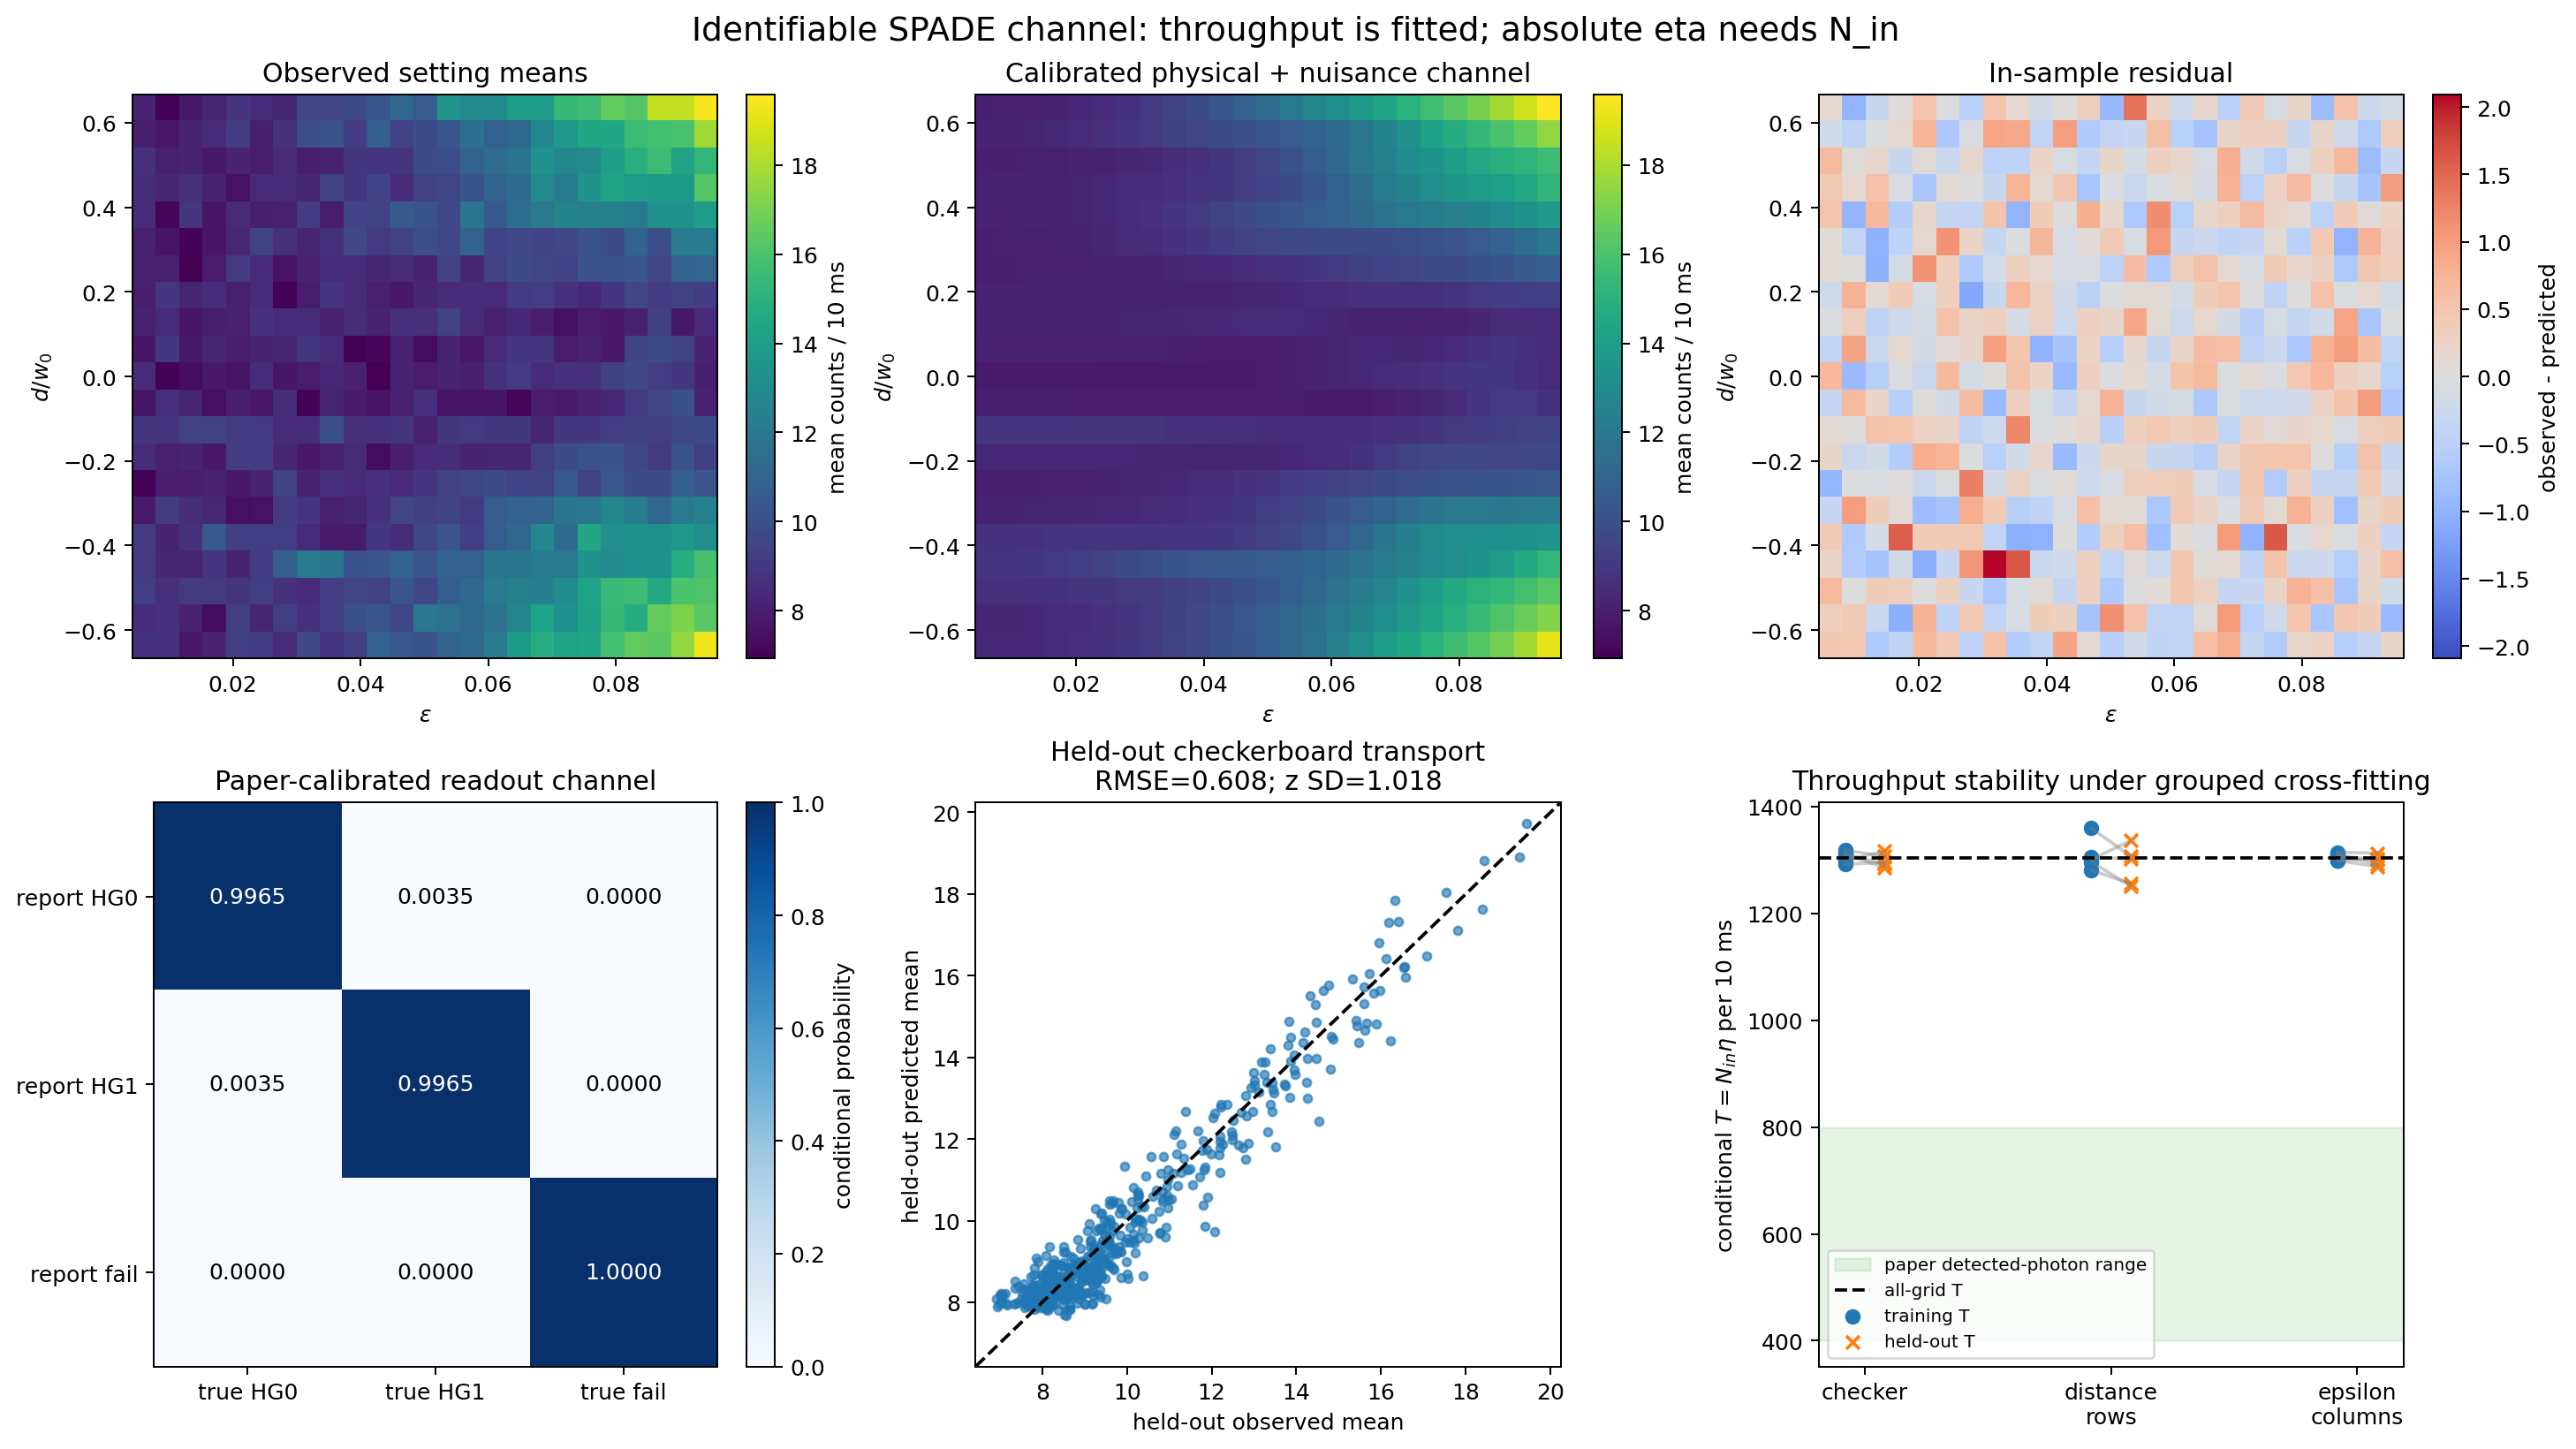
\includegraphics[width=\textwidth]{figures/exoplanets/spade_identifiable_quantum_channel.png}
    \caption{Identifiable sequential-channel fit.  The panels show observed and calibrated setting means, in-sample residuals, the assumed symmetric readout matrix, held-out checkerboard prediction, and the spread of conditional throughput under grouped cross-fitting.  The result is conditional on the fixed readout and zero-mean coupling convention.  It identifies a general throughput scale, not an absolute efficiency.}
    \label{fig:spade_identifiable_channel}
\end{figure}

An independent launched-photon measurement would convert this scale into $\eta=1304.25/N_{\mathrm{in,10\,ms}}$.  Without that measurement, $T$ and $\eta$ must remain distinct.  Background and cross-talk can also compensate for each other and cannot be separated from the aggregate stream.

Random displacement, dephasing, coherent mixing, modal loss, and asymmetric readout are included in a modular sensitivity workbench.  Their example values were not inferred from this dataset.  Appendix~\ref{app:spade_diagnostics} lists every value and its source.  A measured calibration can later replace a provisional value without changing the channel order, fitting method, or QFI pipeline.

% ==============================================================================
\section{Information After the Channels}
\label{sec:spade_qfi_role}
% ==============================================================================

The definitions and numerical methods are those of Chapter~\ref{ch:MathBackground}.  We do not calculate any information quantity by substituting empirical count variance into a QFI formula.  For fixed channel parameters $\boldsymbol\lambda$, the model QFI is
\begin{equation}
    \mathcal{F}_{Q}^{\mathrm{model}}(d_a)
    =\mathcal{F}_{Q}\!\left[
        \widetilde{\rho}_{\mathrm{post}}(d_a,\epsilon;\boldsymbol\lambda)
        \right]
    \label{eq:spade_model_qfi}
\end{equation}
This is the QFI of the assumed pre-measurement state conditional on common survival for estimating $d_a$.  We then calculate the measurement CFI after the stated SPADE and readout maps with the same normalization.  These calculations show where the modeled receiver can lose information.  They do not reconstruct experimental QFI from $n_1$.

\subsection{Conditional information retention}

This calculation asks a simple question.  How much information remains after each stage of the assumed receiver model?  The parameter to be estimated is the separation $d_a$.

These ratios are calculated per surviving photon.  They are not information values per launched photon or per acquisition.  They are also theoretical or conditional results.  The source state and channel parameters are assumed rather than reconstructed from the count data.

The first comparison considers an ideal SPADE receiver that resolves all HG outcomes.  It keeps between $0.99899$ and $1.00000$ of the source QFI.  Full ideal SPADE is therefore almost optimal for this source model.  If the receiver reports only a binary result, $HG_1$ or not $HG_1$, the retained fraction falls to $0.78434$--$0.94485$.  Combining many outcomes into one binary result removes information.

The next comparison limits access to $HG_0$ and $HG_1$, but keeps all other outcomes in a failure flag.  The QFI of this accessible state remains between $0.99777$ and $1.00000$ of the source QFI.  A measurement that separately reports $HG_0$, $HG_1$, and failure keeps $0.99681$--$1.00000$.  Very little information is lost at this stage because the failure probability is kept instead of being discarded.

The largest loss appears after the assumed detector readout cross-talk.  The model uses the symmetric confusion value $\chi=0.0035$ from Eq.~\eqref{eq:spade_readout_matrix}.  After this readout and binary reporting, the retained CFI is only $0.00134$--$0.57026$ of the source QFI.  In this conditional model, detector cross-talk is therefore the main information bottleneck.  Even a small leakage from the bright $HG_0$ port can hide the much weaker separation-dependent signal in the $HG_1$ port.  The damage is strongest near zero separation, where the useful first-order signal is smallest.

The first two ranges use twelve nonzero settings from the measured grid.  The accessible-state and readout ranges use the nine-point test grid listed in Appendix~\ref{app:spade_diagnostics}.  The endpoints should therefore not be compared as if they came from the same setting.  All calculations use the same bright-source-aligned convention and the same per-surviving-photon normalization.  The point $d_a=0$ is excluded because the rank of the source state changes there and requires a separate limiting calculation.

The conclusion is direct.  Ideal SPADE and the flagged low-mode channel preserve almost all the available information.  Binary reporting loses some information.  Under the assumed readout model, detector cross-talk causes the largest loss.  Appendix~\ref{app:spade_diagnostics} gives the setting grids, numerical checks, and full comparison table.

\begin{figure}[htbp]
    \centering
    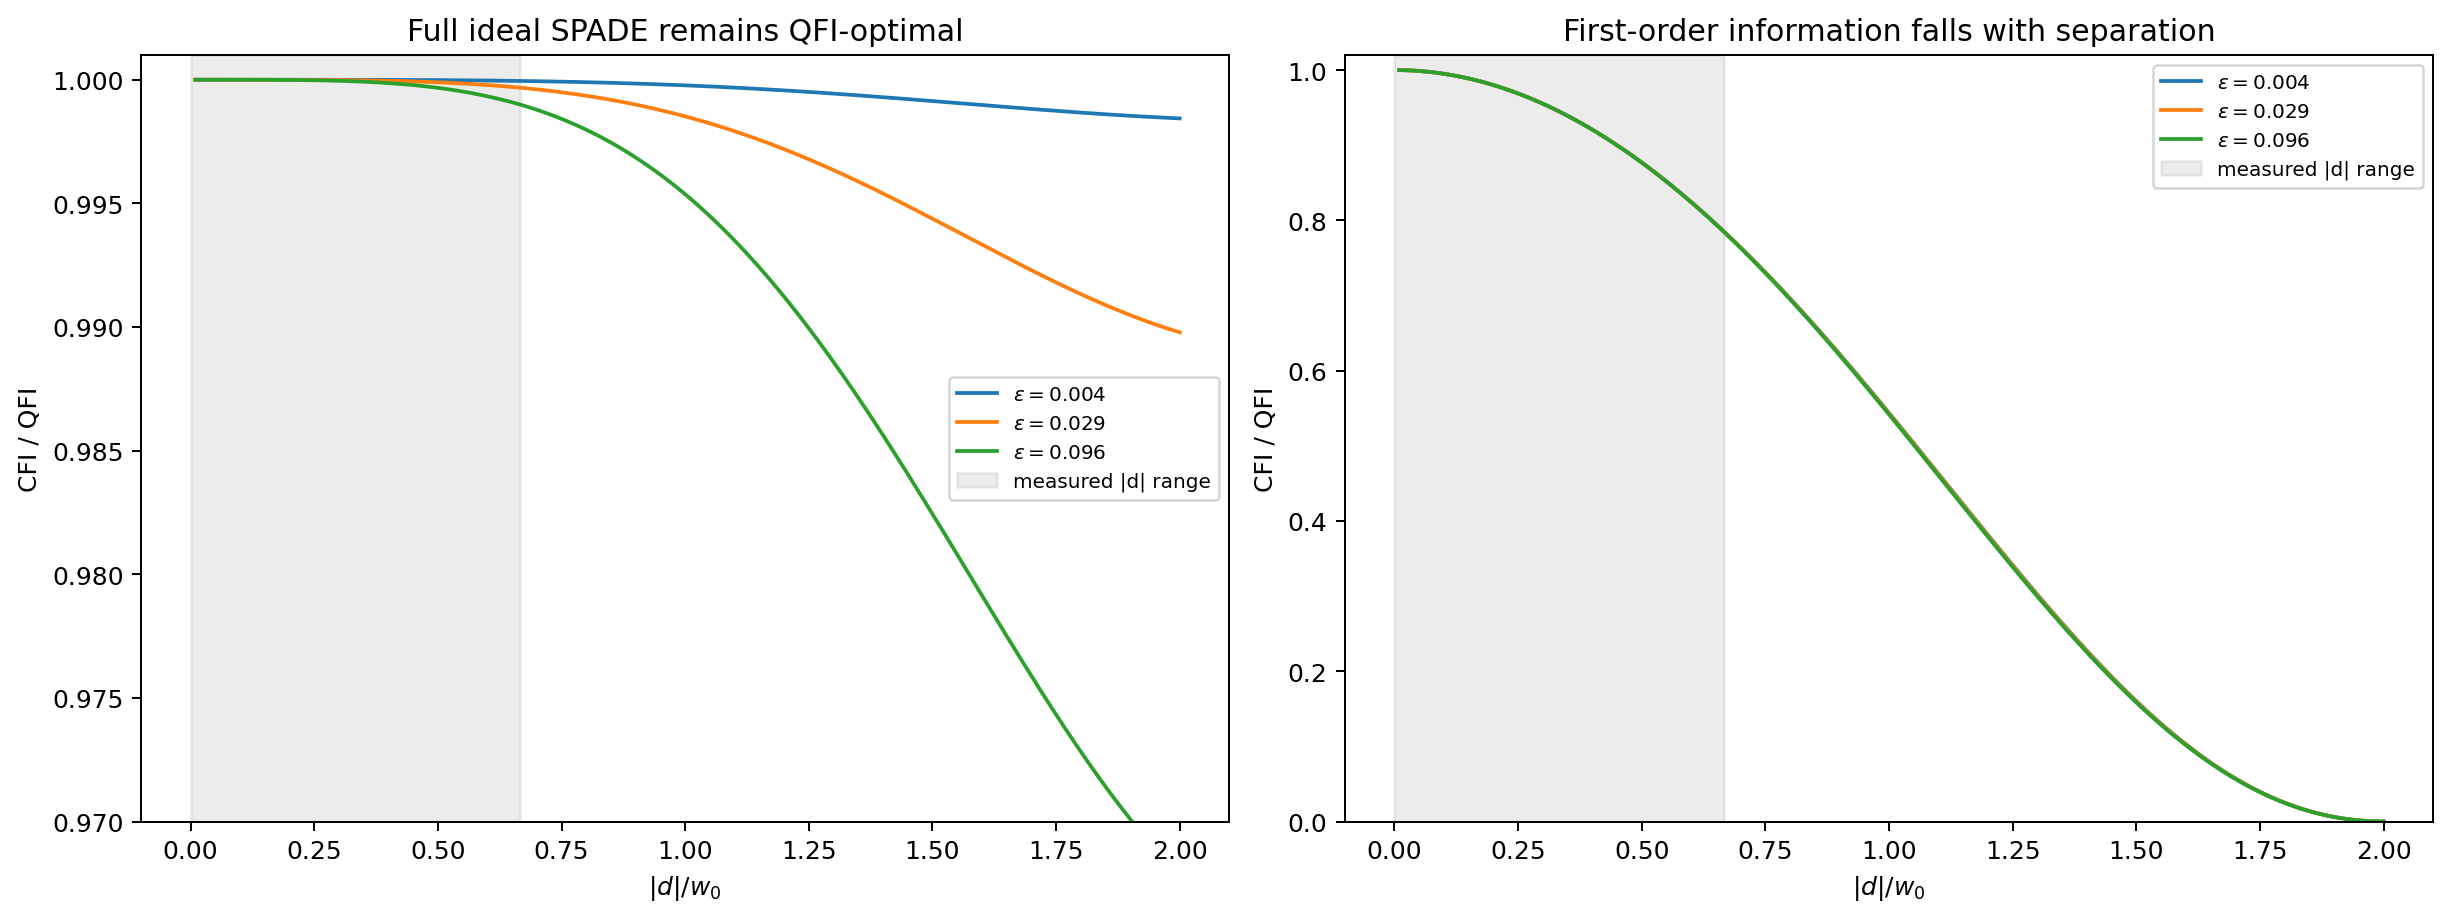
\includegraphics[width=\textwidth]{figures/exoplanets/spade_information_retention.png}
    \caption{Theoretical information retained for the bright-source-aligned model.  The curves compare full ideal SPADE with binary first-order detection at three source fractions.  The grey region marks the measured separation range.  Full ideal SPADE remains almost optimal, while binary detection loses more information as the separation increases.  The values are per surviving photon.}
    \label{fig:spade_information_retention}
\end{figure}


% ==============================================================================
\section{Conclusions and Future Measurements}
\label{sec:spade_conclusions}
% ==============================================================================

\begin{remark}[Scope of the result]
    The hierarchical classical calibration channel predicts held-out $100$-repeat setting means.  Under the stated conventions, the identifiable experimental scale is the conditional throughput $T$, not the efficiency $\eta$.  Full ideal SPADE is nearly QFI-optimal for the assumed source model.  The counts do not reconstruct a density matrix, quantum coherence, the complete channel, or an experimental QFI.
\end{remark}

The most useful next step is a new experiment designed around these limits, possibly in renewed collaboration with ASI Matera.  Separate, time-stamped $HG_{01}$ and $HG_{10}$ streams would resolve directional response and asymmetry.  Simultaneous or interleaved $HG_{00}$ counts, selected higher modes, and a complement or no-click outcome would give modal normalization and preserve the probability outside the measured subspace.

An incident-flux monitor would separate $N_{\mathrm{in}}$ from $\eta$.  Source-blocked runs and detector diagnostics would constrain background and detector effects.  Single-mode injection into every relevant input would determine the readout matrix and modal transmissions.  Independent calibration of $w_0$, $\epsilon$, source position, and sorter alignment would separate nominal coordinates from physical offsets.  Finally, phase-sensitive modal measurements would be needed to constrain coherences, dephasing, and coherent transfer.

With these additions, the measured modal probabilities would first allow calculation of the CFI of the actual SPADE receiver.  Independent coherence-sensitive data or a separately validated channel would then allow comparison with state QFI or TQFI.  Testing VQ-SPADE would also require adaptive optics, i.e., programmable coherent mode transformations, resolved outputs, and the overlap measurements described in Section~\ref{sec:spade_question_record}.  This remains a possible extension for a new experiment, not a claim about the present record.  This order avoids treating population counts as quantum tomography.
